
В данном разделе будут приведены различные примеры запросов на языке ЯЗ.
Описание запроса будет даваться на трех языках: русском, JP-QL, ЯЗ. Также
будет приводиться результат запроса
    \footnote{Если элементом результата запроса является объект, то в таблице с результатом
	приводится его строковое представление.}
    \footnote{Если ячейка в таблице с результатом пуста, то подразумевается, что
	на этом месте находится значение NOT\_DEFINED. Пустое значение (null) указывается явно.}
, полученный на примерах модели, показанной  на рисунках~\ref{fig:model-snapshot-org} и~\ref{fig:model-snapshot-org-spa}.

%\begin{figure}[hbt]
%  \centering
%  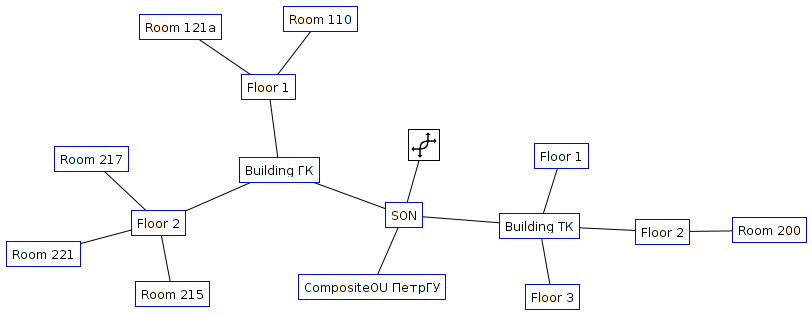
\includegraphics[scale=0.5]{figures/model_snapshot}
%  \caption{Пример пространственной структуры модели Nest}
%  \label{fig:model-snapshot}
%\end{figure}






\subsection{Выборка элементов}
\exastable
    {получить все здания}
    {from Building}
    {building}
    {\begin{tabular}{|l|}
	\hline
	\it{building}\\[5pt]
	\hline
	\hline
	Building ГК\\
	\hline
	Building ТК\\
	\hline
    \end{tabular}}


\exastable
    {получить все здания и для каждого здания указать список его комнат.}
    {select b, r from Building b join b.floors as f join f.rooms as r}
    {building (room)}
    {\begin{tabular}{|l|l|}
	\hline
	\it{building} & \it{room} \\[5pt]
	\hline
	\hline
	Building ГК & Room 110\\
	\cline{2-2}
		    & Room 121a\\
	\cline{2-2}
		    & Room 201\\
	\cline{2-2}
		    & Room 202\\
	\cline{2-2}
		    & Room 203\\
	\cline{2-2}
		    & Room 215\\
	\cline{2-2}
		    & Room 217\\
	\cline{2-2}
		    & Room 221\\
	\hline
	Building ТК & Room 200\\	
	\hline
    \end{tabular}}

\exastable
    {получить все здания и комнаты.}
    {Возможно только с помощью двух разных запросов:
	\begin{itemize}\addtolength{\itemsep}{-0.7\baselineskip}
	    \item from Building
	    \item from Room
	\end{itemize}}
    {building, room}
    {\begin{tabular}{|l|}
	\hline
	\it{building, room}\\[5pt]
	\hline
	\hline
	Building ГК\\
	\hline
	Building ТК\\
	\hline
	Room 215\\
	\hline
	Room 217\\
	\hline
	Room 221\\
	\hline
	Room 110\\
	\hline
	Room 121a\\
	\hline
	Room 200\\
	\hline
	Room 201\\
	\hline
	Room 202\\
	\hline
	Room 203\\
	\hline
    \end{tabular}}

\exastable{найти все здания с их комнатами и все этажи.}
    {Возможно только с помощью двух разных запросов:
	\begin{itemize}\addtolength{\itemsep}{-0.7\baselineskip}
	    \item select b, r from Building b join b.floors as f join f.rooms as r
	    \item from Floor
	\end{itemize}}
    {building (room), floor}
    {\begin{tabular}{|l|l|}
	\hline
	\it{building, floor} & \it{room} \\[5pt]
	\hline
	\hline
	Building ГК & Room 110\\
	\cline{2-2}
		    & Room 121a\\
	\cline{2-2}
		    & Room 215\\
	\cline{2-2}
		    & Room 217\\
	\cline{2-2}
		    & Room 221\\
	\cline{2-2}
		    & Room 201\\
	\cline{2-2}
		    & Room 202\\
	\cline{2-2}
		    & Room 203\\
	\hline
	Building ТК & Room 200\\	
	\hline
	Floor 1 & \\
	\hline
	Floor 2 & \\
	\hline
	Floor 3 & \\
	\hline
	Floor 1 & \\
	\hline
	Floor 2 & \\
	\hline
    \end{tabular}}

\exastable{найти все здания, у каждого здания указать список этажей,
	     а у каждого из этажей указать список комнат.}
    {from Building b join b.floors f join f.rooms}
    {building (floor (room))}
    {\begin{tabular}{|l|l|l|}
	\hline
	\it{building} & \it{floor} & \it{room}\\[5pt]
	\hline
	\hline
	Building ГК & Floor 1 & Room 110\\
	\cline{3-3}
		    & & Room 121a \\
	\cline{2-3}
		    & Floor 2 & Room 215\\
	\cline{3-3}
		    & & Room 217\\
	\cline{3-3}
		    & & Room 201\\
	\cline{3-3}
		    & & Room 202\\
	\cline{3-3}
		    & & Room 203\\
	\cline{3-3}
		    & & Room 221\\
	\hline
	Building ТК & Floor 1 & \\	
	\cline{2-3}
		    & Floor 2 & Room 200\\
	\cline{2-3}
		    & Floor 3 & \\
	\hline
    \end{tabular}}

\exastable{найти все здания, у каждого здания указать список этажей и комнат}
    {невозможно}
    {building (floor, room)}
    {\begin{tabular}{|l|l|}
	\hline
	\it{building} & \it{floor, room} \\[5pt]
	\hline
	\hline
	Building ГК & Floor 1\\
	\cline{2-2}
		    & Floor 2\\
	\cline{2-2}
		    & Room 110\\
	\cline{2-2}
		    & Room 121a\\
	\cline{2-2}
		    & Room 215\\
	\cline{2-2}
		    & Room 217\\
	\cline{2-2}
		    & Room 221\\
	\cline{2-2}
		    & Room 201\\
	\cline{2-2}
		    & Room 202\\
	\cline{2-2}
		    & Room 203\\
	\hline
	Building ТК & Floor 1\\	
	\cline{2-2}
		    & Floor 2\\
	\cline{2-2}
		    & Floor 3\\
	\cline{2-2}
		    & Room 200\\
	\hline
    \end{tabular}}


\exastable
    {для каждой простой организационной единицы  получить всю иерархию вышестоящих отделов.}
    {невозможно}
    {simpleou.parent+}
    {\begin{tabular}{|l|l|}
	\hline
	\it{parent} & \it{parent}\\[5pt]
	\hline
	\hline
	IT-Отдел & ПетрГУ \\
	\hline
	IT-Отдел & ПетрГУ \\
	\hline
	ОргОтдел & ПетрГУ \\
	\hline
	МатФак & ПетрГУ \\
	\hline
    \end{tabular}}

\exastable
    {для каждой простой организационной единицы получить всю иерархию  вышестоящих отделов.
    В результат запроса включить саму организационную единицу.}
    {невозможно}
    {simpleou.parent*}
    {\begin{tabular}{|l|l|l|}
	\hline
	\it{simpleou} & \it{parent} & \it{parent}\\[5pt]
	\hline
	\hline
	1C автоматизация & IT-Отдел & ПетрГУ \\
	\hline
	Отдел безопасности & IT-Отдел & ПетрГУ \\
	\hline
	По международным связям & ОргОтдел & ПетрГУ \\
	\hline
	Кафедра ИМО & МатФак & ПетрГУ \\
	\hline
    \end{tabular}}


\exastable
    {показать всю иерархию организационных единиц для всех сложных организационных единиц.}
    {невозможно}
    {compositeou.ous*}
    {\begin{tabular}{|l|l|l|}
	\hline
	\it{compositeou} & \it{ous} & \it{ous}\\[5pt]
	\hline
	\hline
	ПетрГУ &  ЮрОтдел & \cl{null} \\
	\cline{2-3}
		    & ОргОтдел & По международным \\
		    & & связям \\
	\cline{3-3}
		    &	       & Пресс-Служба \\
	\cline{2-3}
		    & IT-Отдел & Отдел безопасности\\
	\cline{3-3}
		    &	       & 1C автоматизация \\
	\cline{2-3}
		    & МатФак & Кафедра ИМО \\
	\hline
	ОргОтдел & По международным связям & \cl{null} \\
	\cline{2-3}
		& Пресс-Служба & \cl{null} \\
	\hline
	IT-Отдел & Отдел безопасности & \cl{null} \\
	\cline{2-3}
		& 1C автоматизация & \cl{null} \\
	\hline
	ЮрОтдел & \cl{null} & \cl{null} \\
	\hline
	Пресс-Служба & \cl{null} & \cl{null} \\
	\hline
	МатФак & Кафедра ИМО & \cl{null} \\
	\hline
    \end{tabular}}







\subsection{Ограничения}
\exastable
    {найти здание главного корпуса.}
    {from Building b where b.name='ГК'}
    {building.name=``ГК''}
    {\begin{tabular}{|l|l|}
	\hline
	\it{building, floor} \\[5pt]
	\hline
	\hline
	Building ГК\\
	\hline
	\end{tabular}}

\exastable
    {найти все здания, в которых есть комната с номером 215.}
    {select b \\ 
	& \hspace{0.4cm} from Building b join b.floors f join f.rooms r \\ 
	& \hspace{0.4cm} where r.number='215'}
    {building.room.number=``215''}
    {\begin{tabular}{|l|l|}
	\hline
	\it{building} \\[5pt]
	\hline
	\hline
	Building ГК\\
	\hline
    \end{tabular}}

\exastable
    {вывести список зданий и для каждого здания указать список комнат, 
	номера которых начинаются с последовательности ``21''.}
    {невозможно}
    {building (room.number\symbol{"7E}``21.*'')}
    {\begin{tabular}{|l|l|}
	\hline
	\it{building} & \it{room} \\[5pt]
	\hline
	\hline
	Building ГК & Room 215\\
	\cline{2-2}
		    & Room 215\\
	\cline{2-2}
		    & Room 217\\
	\hline
	Building ТК & \cl{null}\\	
	\hline
    \end{tabular}}

\exastable
    {вывести список зданий, в которых есть комнаты, 
	номера которых начинаются с последовательности ``21''. 
	Для каждого здания вывести полный список комнат.}
    {невозможно}
    {building.room.number\symbol{"7E}``21.*'' (room)}
    {\begin{tabular}{|l|l|}
	\hline
	\it{building} & \it{room} \\[5pt]
	\hline
	\hline
	Building ГК & Room 110\\
	\cline{2-2}
		    & Room 121a\\
	\cline{2-2}
		    & Room 201\\
	\cline{2-2}
		    & Room 202\\
	\cline{2-2}
		    & Room 203\\
	\cline{2-2}
		    & Room 215\\
	\cline{2-2}
		    & Room 217\\
	\cline{2-2}
		    & Room 221\\
	\hline
    \end{tabular}}

\exastable
    {вывести список зданий, в которых есть комнаты, 
	номера которых начинаются с последовательности ``21''. 
	Для каждого здания вывести список этих комнат.}
    {невозможно}
    {building.room.number\symbol{"7E}``21.*'' (room.number\symbol{"7E}``21.*'')}
    {\begin{tabular}{|l|l|}
	\hline
	\it{building} & \it{room} \\[5pt]
	\hline
	\hline
	Building ГК & Room 215\\
	\cline{2-2}
		    & Room 215\\
	\cline{2-2}
		    & Room 217\\
	\hline
    \end{tabular}}


\exastable
    {найти номера комнат на первом этаже главного корпуса.}
    {select r.number from Room r\\ &
	\hspace{0.4cm} where r.floor.number=1 and r.floor.building.name='ГК'}
    {room[number].(floor.number=1 \&\& building.name=``ГК'')}
%    {room\#r.number (:where r.floor.number=1 \&\& r.floor.building.name=``ГК'')}
    {\begin{tabular}{|l|}
	\hline
	\it{room.number}\\[5pt]
	\hline
	\hline
	110 \\
	\hline
	121a \\
	\hline
	\end{tabular}}

\exastable
    {показать всю иерархию организационных единиц, в имени которых 
	встречается слово ``Отдел'', для всех сложных организационных единиц.}
    {невозможно}
    {compositeou.ous*.name\symbol{"7E}``.*Отдел.*''}
    {\begin{tabular}{|l|l|l|}
	\hline
	\it{compositeou} & \it{ous} & \it{ous}\\[5pt]
	\hline
	\hline
	ПетрГУ &  ЮрОтдел & \cl{null} \\
	\cline{2-3}
		    & ОргОтдел & По международным \\
		    & & связям \\
	\cline{3-3}
		    &	       & Пресс-Служба \\
	\cline{2-3}
		    & IT-Отдел & Отдел безопасности\\
	\cline{3-3}
		    &	       & 1C автоматизация \\
	\cline{2-3}
		    & МатФак & Кафедра ИМО \\
	\hline
	IT-Отдел & Отдел безопасности & \cl{null} \\
	\cline{2-3}
		& 1C автоматизация & \cl{null} \\
	\hline
    \end{tabular}}







\subsection{Вызов функции}
\exastable
    {подсчитать количество комнат.}
    {select count(r) from Room r}
    {@count(room)}
    {\begin{tabular}{|l|l|}
	\hline
	\it{count} \\[5pt]
	\hline
	\hline
	9\\
	\hline
    \end{tabular}}

\exastable
    {получить все здания и подсчитать количество комнат в них.}
    {select b.id, count(r) \\ 
	& \hspace{0.4cm} from Building b join b.floors as f join f.rooms as r \\
	& \hspace{0.4cm} group by b.id}
    {building (@count(room))}
    {\begin{tabular}{|l|l|}
	\hline
	\it{Building} & \it{count}\\[5pt]
	\hline
	\hline
	Building ГК & 8\\
	\hline
	Building ТК & 1\\
	\hline
    \end{tabular}\\[10pt]
    \bf{Замечание:} & Обратите внимание, что набор объектов \cl{Room} определяется относительно 
	объекта \cl{Building}, так как \cl{Room} определяется в скобках относительно \cl{Building},
	то есть для каждого объекта \cl{Building} будет найден список связанных с ним \cl{Room} и 
	передан в функцию \cl{count}.
	Запрос \query{building, @count(room)} вначале выведет весь список \cl{Building}, а затем 
	результат функции со списком всех объектов \cl{Room}.\\
	& Также стоит заметить, что запрос на JP-QL не совсем соответствет запросу пользователя. 
	JP-QL не может вернуть сами объекты-зданий, а возвращает только его идентификатора.
	Эта проблема связана в возможностями группировки JP-QL.}

\exastable
    {вывести список всех зданий с количеством комнат, а также указать количество зданий.}
    {Возможно с помощью двух запросов:
	\begin{itemize}\addtolength{\itemsep}{-0.7\baselineskip}
	    \item select b.id, count(r) 
	    from Building b join b.floors as f join f.rooms as r
	    group by b.id
	    \item select count(b) from Building b
	\end{itemize}
    }
    {building (@count(room)), @count(building)}
    {\begin{tabular}{|l|l|}
	\hline
	\it{building, count} & \it{count}\\[5pt]
	\hline
	\hline
	Building ГК & 5\\
	\hline
	Building ТК & 1\\
	\hline
	2 & \\
	\hline
    \end{tabular}}

\exastable
    {найти этаж с наибольшим номером в здании главного корпуса.}
    {select f from Floor f \\ & 
	where f.number in (select max(f.number) from Floor f where f.building.name='ГК') \\ &
	and f.building.name='ГК'}
    {@first(floor.number=(@max(building.(name=``ГК'').floor.number) 
	\\ & \&\& building.name=``ГК''))}
    {\begin{tabular}{|l|}
	\hline
	\it{floor} \\[5pt]
	\hline
	\hline
	Floor 2 \\
	\hline
    \end{tabular} \\
    \bf{Замечание:} & Вызов функции \cl{@first} необходим для получения только одного
	объекта этажа. Так как модель не предполагает ограничений на количество этажей с одинаковым
	номером в одном здании, то без вызова \cl{@first} запрос вернет весь список этажей с 
	максимальным номером.}






\subsection{Группировка}
\exastable
    {выбрать все этажи, сгруппировав их по номерам.}
    {невозможно}
    {floor:number}
    {\begin{tabular}{|l|}
	\hline
	\it{floor:number}\\[5pt]
	\hline
	\hline
	[Floor 1, Floor 1]\\
	\hline
	[Floor 2, Floor 2]\\
	\hline
	[Floor 3]\\
	\hline
    \end{tabular}}

\exastable
    {выбрать все этажи, сгруппировав их по номерам и вывести список их комнат.}
    {невозможно}
    {floor:number (room)}
    {\begin{tabular}{|l|l|}
	\hline
	\it{floor:number} & \it{room}\\[5pt]
	\hline
	\hline
	[Floor 1, Floor 1] & Room 110 \\
	\cline{2-2}
		& Room 121a \\
	\hline
	[Floor 2, Floor 2] & Room 215 \\
	\cline{2-2}
		& Room 217 \\
	\cline{2-2}
		& Room 221 \\
	\cline{2-2}
		& Room 201 \\
	\cline{2-2}
		& Room 202 \\
	\cline{2-2}
		& Room 203\\
	\cline{2-2}
		& Room 200 \\
	\hline
	[Floor 3] & \\
	\hline
    \end{tabular}}


\exastable
    {выбрать все этажи, сгруппировав их по номерам и подсчитать количество комнат по полученным группам.}
    {невозможно}
    {floor:number (@count(room))}
    {\begin{tabular}{|l|l|}
	\hline
	\it{floor:number} & \it{count}\\[5pt]
	\hline
	\hline
	[Floor 1, Floor 1] & 2 \\
	\hline
	[Floor 2, Floor 2] & 7 \\
	\hline
	[Floor 3] & 0 \\
	\hline
    \end{tabular}}

\exastable
    {показать номер этажа и количество комнат на этажах с этим номером.}
    {select f.number, count(r) \\
    & \hspace{0.4cm} from Floor f join f.rooms r \\
    & \hspace{0.4cm} group by f.number}
    {floor:(number) (@count(room))}
    {\begin{tabular}{|l|l|}
	\hline
	\it{number} & \it{count}\\[5pt]
	\hline
	\hline
	1 & 2 \\
	\hline
	2 & 7 \\
	\hline
	3 & 0 \\
	\hline
    \end{tabular}}

\exastable
    {вывести список зданий и их комнат, сгруппировав комнаты по этажу.}
    {невозможно}
    {building (room:floor)}
    {\begin{tabular}{|l|l|}
	\hline
	\it{building} & \it{room:floor}\\[5pt]
	\hline
	\hline
	Building ГК & [Room 110, Room 121a] \\
	\cline{2-2}
		    & [Room 215, Room 217, Room 221, \\
		    & Room 201, Room 202, Room 203] \\
	\hline
	Building ТК & [] \\
	\cline{2-2}
		    & [Room 200] \\
	\cline{2-2}
		    & [] \\
	\hline
    \end{tabular}\\
    \bf{Замечание:} & Наличие пустых списков связано с тем, что в примере модели для здания \cl{Building ТК}
	на этажа \cl{Floor 1} и \cl{Floor 3} нет комнат.
    }





\subsection{Сортировка}
\exastable
    {получить список комнат, упорядочив его по убыванию номера комнаты.}
    {from Room r order by r.number desc}
    {room\{desc:number\}}
    {\begin{tabular}{|l|}
	\hline
	\it {room} \\
	\hline
	\hline
	Room 221 \\
	\hline
	Room 217 \\ 
	\hline
	Room 215 \\
	\hline
	Room 203 \\
	\hline
	Room 202 \\
	\hline
	Room 201 \\
	\hline
	Room 200 \\
	\hline
	Room 121a \\
	\hline
	Room 110 \\	
	\hline
    \end{tabular}}

\exastable
    {выбрать этажи, указав у каждого этажа его список комнат. Этажи отсортировать 
    по номеру в порядке убывания, а комнаты по номеру в порядке возрастания.}
    {select r.floor, r from Room r order by r.floor.number desc, r.number asc}
    {floor\{desc:number\} (room\{asc:number\})}
    {\begin{tabular}{|l|l|}
	\hline
	\it {floor} & room\\
	\hline
	\hline
	Floor 2 & Room 200 \\
	\cline{2-2}
		& Room 201 \\ 
	\cline{2-2}
	    & Room 202 \\
	\cline{2-2}
	    & Room 203 \\
	\cline{2-2}
	    & Room 215 \\
	\cline{2-2}
	    & Room 217 \\
	\cline{2-2}
	    & Room 221 \\
	\hline
	Floor 1 & Room 110 \\
	\cline{2-2}
		& Room 121a \\	
	\hline
    \end{tabular}}

\exastable
    {выбрать все комнаты, отсортировав их сначала по номеру этажа в 
    порядке убывания, а затем по номеру в порядке возрастания.}
    {select r from Room r order by r.floor.number asc, r.number desc}
    {room\{asc:floor.number desc:number\}}
    {\begin{tabular}{|l|}
	\hline
	\it{room}\\
	\hline
	\hline
	Room 121a \\
	\hline
	Room 110 \\
	\hline
	Room 221 \\
	\hline
	Room 217 \\ 
	\hline
	Room 215 \\
	\hline
	Room 203 \\
	\hline
	Room 202 \\
	\hline
	Room 201 \\
	\hline
	Room 200 \\	
	\hline
    \end{tabular}}

\exastable
    {}
    {}
    {}
    {

    }


